\let\negmedspace\undefined
\let\negthickspace\undefined
\documentclass[journal]{IEEEtran}
\usepackage[a5paper, margin=10mm, onecolumn]{geometry}
%\usepackage{lmodern} % Ensure lmodern is loaded for pdflatex
\usepackage{tfrupee} % Include tfrupee package

\setlength{\headheight}{1cm} % Set the height of the header box
\setlength{\headsep}{0mm}     % Set the distance between the header box and the top of the text

\usepackage{gvv-book}
\usepackage{gvv}
\usepackage{cite}
\usepackage{amsmath,amssymb,amsfonts,amsthm}
\usepackage{algorithmic}
\usepackage{graphicx}
\usepackage{textcomp}
\usepackage{xcolor}
\usepackage{txfonts}
\usepackage{listings}
\usepackage{enumitem}
\usepackage{mathtools}
\usepackage{gensymb}
\usepackage{comment}
\usepackage[breaklinks=true]{hyperref}
\usepackage{tkz-euclide} 
\usepackage{listings}
% \usepackage{gvv}                                        
\def\inputGnumericTable{}                                 
\usepackage[latin1]{inputenc}                                
\usepackage{color}                                            
\usepackage{array}                                            
\usepackage{longtable}                                       
\usepackage{calc}                                             
\usepackage{multirow}                                         
\usepackage{hhline}                                           
\usepackage{ifthen}                                           
\usepackage{lscape}
\begin{document}

\bibliographystyle{IEEEtran}
\vspace{3cm}

\title{1.1.5.10}
\author{AI24BTECH11022 - Pabbuleti Venkata Charan Teja}
\maketitle

\renewcommand{\thefigure}{\theenumi}
\renewcommand{\thetable}{\theenumi}

\textbf{Question:}\\
Find the ratio in which the line segment joining the points $A(1,-5)$ and $B(-4,5)$ is divided by the $x$-axis. Also, find the coordinates of the point of division.

\hfill{(10,2021)}

\textbf{Solution:}

\begin{table}[h!]
\renewcommand{\thetable}{1}
    \centering
   \begin{tabular}{|c| c |}
\hline
\textbf{Variable} & \textbf{Value} \\
\hline
$A$ & \myvec{1 \\ -5\\}\\
\hline
$B$ & \myvec{-4 \\ 5\\}\\
\hline
$k:1$    & Ratio in which the line $AB$ is divided by $x$-axis \\
\hline
$X$  & Point of division of $A$ , $B$\\
\hline
\end{tabular} 
   \def\tablename{Table}
   \caption{Variables Used}
    \label{tab1.1.5.10.1}
\end{table}
If $X$ divides $AB$ in the ratio k:1,

\begin{align}
X=\frac{kB+A}{k+1} \label{eq1.1.5.10.1} \\
X=\frac{1}{k+1}
\myvec{
-4k+1 \\
5k-5 \\
} \label{eq1.1.5.10.2} \\
X=
\myvec{
x \\
y \\
} \\
X=x\myvec{1 \\ 0 \\}+y\myvec{0 \\ 1 \\} \label{eq1.1.5.10.3}\\
X=
\myvec{
1 & 0 \\
0 & 1 \\
}
\myvec{
x \\
y \\
}\label{eq1.1.5.10.4} \\
\implies
\myvec{
1 & 0 \\
0 & 1 \\
}
\myvec{
x \\
y \\
}
=\frac{1}{k+1}
\myvec{
-4k+1 \\
5k-5 \\
} \label{eq1.1.5.10.5}
\end{align}

But as $X$ is on $x$-axis,
\begin{align}
y=0\\
\frac{5k-5}{k+1}=0 \label{eq1.1.5.10.6} \\
5k-5=0 \label{eq1.1.5.10.7} \\
k=1 \label{eq1.1.5.10.8}
\end{align}

$\therefore$ The ratio in which the line is divided by $x$-axis is $1:1$ \\
The coordinates of the point of the division is \\
\begin{align}
\myvec{
x \\
y \\
}
=\frac{1}{k+1}
\myvec{
-4k+1 \\
5k-5 \\
} \label{eq1.1.5.10.9}
\\
\myvec{
x \\
y\\
}
=\frac{1}{2}
\myvec{
-3 \\
0 \\
} \label{eq1.1.5.10.10}
\\
\myvec{
x \\
y \\
}
=
\myvec{
\frac{-3}{2} \\
0 \\
} \label{eq1.1.5.10.11}
\end{align}

$\therefore$ The point of division $\brak{x,y}=\brak{\frac{-3}{2},0}$

\begin{figure}[h!]
\renewcommand{\thefigure}{1}
    \centering
    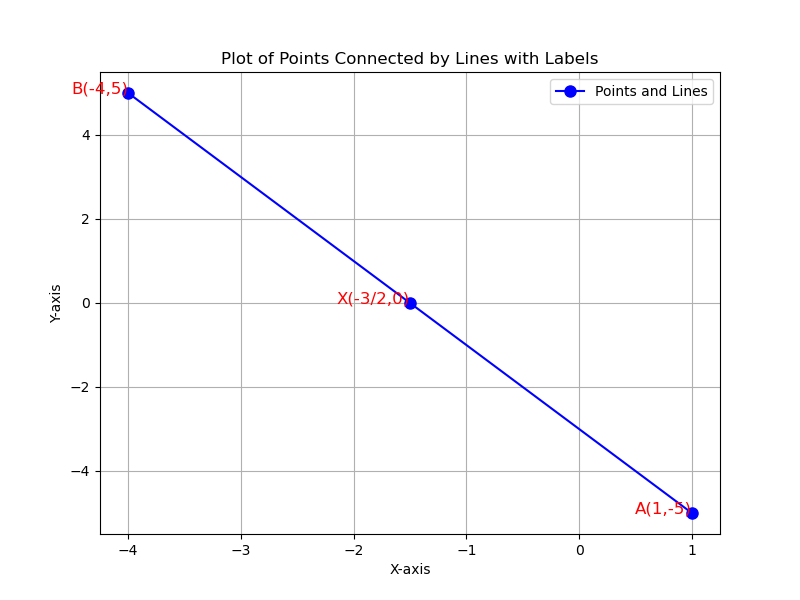
\includegraphics[width=0.7\linewidth]{figs/Figure_1.png}
    \caption{Plot of the points}
    \label{fig1.1.5.10.1}
\end{figure}

\end{document}
